% Quality Metrics
\begin{tikzpicture}
    \node [mybox] (box){%
        \begin{minipage}{0.48\textwidth}
        \begin{tabular}{lp{0.8\textwidth} l}
            Metric & Description \\
            \hline
            Relevance & Ability of recommending items that the user likes \\
            Coverage & Ability of recommending items that the user has not seen \\
            Novelty & Ability of recommending unknown items \\
            Diversity & Ability of recommending different items \\
            Consistency & Ability to give consistent recommendations \\
            Confidence & Measure how much the model is sure about its recommendations \\
            Serendipity & Ability of recommending unexpected items \\
        \end{tabular}
        \end{minipage}
    };

% --- Quality Metrics header ---
\node[fancytitle, right=10pt] at (box.north west) {Quality Metrics};
\end{tikzpicture}

% --- Classification Metrics ---
\begin{tikzpicture}
    \node [mybox] (box){%
        \begin{minipage}{0.48\textwidth}
        \begin{center}
            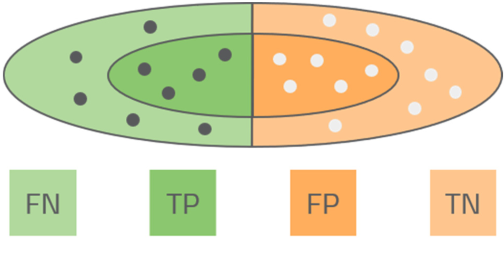
\includegraphics[height=0.1\textheight]{imgs/02_metrics.png}
        \end{center}
        \begin{tabular}{lp{0.8\textwidth} l}
            Metrics & Formula \\
            \hline
            Recall & $\frac{TP}{FN + TP}$ 
            \\
            
            Precision & $\frac{TP}{TP + FP}$ 
            \\
            
            Fallout & $\frac{FP}{FP + TN}$ 
            \\
            
            AUC & $\frac{\sum_{k} Recall(k) \cdot \Delta Fallout}{N_i}$ 
            \\
            
            AP & $\sum_{k} Precision(k) \cdot [Recall(k) - Recall(k - 1)]$ 
            \\

            MAP & $\frac{\sum_u AP_u(k)}{N_u}$
        \end{tabular}
        \end{minipage}
    };

% --- Classification Metrics header ---

\node[fancytitle, right=10pt] at (box.north west) {Classification Metrics};

\end{tikzpicture}